%!TEX root = ../report.tex

% 
% Objectives
% 

\section{Concepts}
\label{Concepts}

This section discusses key aspects of Facilities Management, Benchmarking and Cloud applications.

\subsection{Facilities Management}
\label{FacilitiesManagement}

Core activities are bound to the central business of the organization and its strategy. While the non-core activities are not necessarily required by an organization in fulfilling its value proposition to its customers, and can be outsourced to third parties (such as security, payroll, cleaning, maintenance of the building, catering, printing, vehicle maintenance or conference facilities). 

Facility Management (FM) is a non-core activity that supports an organization in the pursuit of its objectives (core business), and is considered ``the practice of coordinating the physical of business administration, architecture, behaviour and engeneering science" \cite{IFMA} by the International Facility Management Association (IFMA). FM is a result-oriented management of facilities and services securing best value in the provision of services, making the organization more efficient, by giving better conditions and making less expenditures.

FM is supported by specialized software such as Computer Aided Facility Management (CAFM) packages that track space usage, cable pathways, employee locations, security and access control.

CAFM systems are often integrated with Computer Aided Design (CAD), important to support the planning and monitoring of spaces and activities in it, and a database back-end that contains non graphical data about the spaces. CAFM software also enables managing changes to the space since can be tried and tested in computer before they are made, which can avoid future problems. 
CAFM systems can be populated from Building Information Models (BIM) information containing geometry, spatial relationships, geographic information, quantities and component properties \cite{Atkin2009}, also interfaces to other systems such as a Computerized Maintenance Management Systems (CMMS) to manage preventive maintenance activities. They also have the ability to help decrease the time for task request to task completion, increase the speed and accuracy of information related to each task, and provide improved cost and trend analysis \cite{May2012}. 

These systems bring along several benefits as: 
\begin{enumerate*}[label=\itshape\roman{enumi})]
	\item efficient completion of operational sequences (entry and analysis of data),
	\item increase the productivity of workers (by determining property improvements),
	\item potential cost savings (in areas such as cleaning contracts and energy consumption),
	\item analysis of information on costs,
	\item supporting management decisions, 
	\item precise valuation of fixed assets,
	\item optimization of space utilization.
\end{enumerate*}

Beyond this type of software, there are others like Incident Management Systems (IMS) that are used by operators (which register incidents) or technicians (who deal with occurrences and close them) to register, centralize and follow each occurrence's status. These systems can generate an automatic work backlog for each technician, which provides work efficiency. It also has reporting services, statistics, incidents status, etc. IMS can be integrated with CMMS or with incident management systems from third party service suppliers to fill-in work order requests.

Computerized Maintenance Management Systems (CMMS) creates and associates maintenance plans, that can be grouped by type of device, for each equipment of an organization, such as air conditioning, roller stairs, furnitures, etc. Some CMMS assist in performing contract management and equipment management. Some of CMMS can be integrated with BAS to obtain equipment usage metrics, however some information can not be possible to retrieve directly from BAS, but it is possible using gathering devices.

Building Automation Systems manage every building's environment aspect, automatically controlling devices installed in the building. Facility managers can remotely command and supervise automation sub-systems in real-time. BAS keeps a history log of the status of each device and defines alarm conditions that can be used to detect malfunction symptoms or devices failure, and can be integrated to CMMS or CAFM tools to report space usage metrics obtained from occupancy sensors.

Energy Management Systems (EMS) gathers all energy consumption information from energy meter devices installed along the building such as electric current consumption. This information can be analyzed in detail and enables facility managers to analyze consumption variation within comparable periods of time. BAS and EMS can be connected together to create consumption profiles and determine relative contribution of devices or groups of devices to the overall energy consumption.

However Enterprise Resource Planning (ERP) systems are not considered FM applications, they are very important on FM environment where management of suppliers, logistics, accounting, billing and orders is being made. 

Integrated Workspace Management System (IWMS) suites integrate functionalities of an ERP for FM with CAFM and CMMS in one single application. The organization of all these softwares referred above can be seen on Figure \ref{fig:ClassesFMApps}.

\begin{figure}[t!]
  \centering
  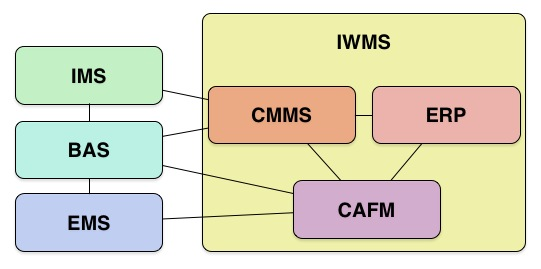
\includegraphics[width=0.95\textwidth]{img/ClassesFMApps.jpg}
  \caption{Organization of the six classes of software applications for FM. The interoperability between the classes is represented by a line between them. IWMS is a group composed by the three classes: CMMS, ERP and CAFM.}
  \label{fig:ClassesFMApps}
\end{figure}

Most of these systems today are web-based enabling an easier entering of the facilities data that can be analyzed and consulted anywhere. These analysis and benchmarking of all data results in Key Performance Indicators (KPIs) over a core of skills that are aligned with business objectives as a way to measure current levels of performance and achievement. 

\subsection{Benchmarking}

Benchmarking has been defined has the search of ``industry best practices that lead to superior performance" by Camp \cite{Camp1989}. It is an important process to compare performance aspects such as operating costs, maintenance and cleaning activities, space utilization, energy consumption or administrative costs. It uses different previously established metrics, identifies differences, alternative approaches and assess opportunities for improvements and change. Overall, it is a process that gives organizations instruments to know how they are performing both internally and to costumers.
 
Benchmarking can bring many advantages for a facility such as:
\begin{enumerate*}[label=\itshape\roman{enumi})]
	\item not waste time and costs when someone else has already done it better, faster and cheaper,
	\item increase the velocity of change and restructuring,
	\item improvement in and off itself, by forcing organizations to examine present processes,
	\item more likely implementation, because process owners are more involved.
\end{enumerate*}

Historically FM started with a focus on performance measurement, that had three broad purposes: 
\begin{enumerate*}[label=\itshape\roman{enumi})]
	\item ensure the achievement of goals and objectives, 
	\item evaluate, control and improve procedures and processes, 
	\item compare and assess the performance of different organizations, teams and individuals. 
\end{enumerate*}

Over the years, however, attentions shifted to quality and consumer satisfaction \cite{Pitt2008}, for this end, benchmark has a set of goals such as better prioritize and allocate resources, and identify opportunities, but it has a major goal: performance improvement of the organization. To this end, there is a set of requirements such as:
 \begin{enumerate*}[label=\itshape\roman{enumi})]
	\item know what clients require for the organization process,
	\item key stakeholders have to be involved in the benchmarking process,
	\item there can not be change resistance,
	\item results are not instantaneously.
\end{enumerate*}

% The focus of FM skills and techniques should be in the area that contributes to the overall management of a business by relating accommodation and support infrastructure issues to business, financial and personal criteria \cite{Pitt2008}. There is a need to assess performance in order to guide management decision-making (performance measurement is a driver to an innovation process in an organization). 

Benchmarking is not as simples as the aggregation of a few indicators. There must be meaning for each one of them, a purpose for choosing each one. Camp lists four fundamental steps for benchmarking \cite{Camp1989}:
\begin{itemize}
	\item {\bf Knowing operation} to evaluate internal operation strengths and weaknesses.
	\item {\bf Knowing the industry leaders or competitors} to know the strengths and weaknesses of the competition.
	\item {\bf Incorporating the best} to emulate the strengths of the leaders in competition.
	\item {\bf Gaining superiority} to go beyond the best practices installed and be the best of the best.
\end{itemize}

Clearly, the FM benchmarking process requires a planning phase that decides which data to collect \cite{Gilleard2004}.

\subsection{Key Performance Indicators}

Performance Indicators are collected in many complex systems which, such as education, deliver a service \cite{Fitz-Gibbon1990}. These indicators are not perfect measures, without error or problems of definition and interpretation, but they are important pointers to the functioning of the system and keeping track of them is one aspect of quality control \cite{Fitz-Gibbon1990}.

The first step of benchmarking is the establishment of performance objectives and metrics. For example, the number of tasks completed in a given time interval. Just like all the actions that must be well performed to accomplish satisfactorily those objectives or goals. All these are important for all measurements and performance comparison between benchmarking parties, but it is important to know that the choosing of wrong indicators can be damaging, and therefore, it is also important to know that Measurements and Indicators are distinct concepts. Measurements are a direct representation of the scale of the organization and are direct measurable items (for organizations internal usage) while Indicators are quantifiable metrics that reflects organizations goals achievement (external usage). It is important to distinguish Performance Indicators (PI) from Key Performance Indicators (KPI). The PIs tells you what to do, while the KPIs tells you what to do to increase performance dramatically, so, they represent a set of measures focusing on most critical aspects of organizational performance for the current and future success of the organization \cite{Parmenter2007}.

KPIs are not the same for all the sectors and employees on an organization. Associated directors or head of advisors have custom KPI for their specific responsibilities. Also, there are various generic KPIs for other professionals and managerial personel based on business measures. However, they all must be SMART \cite{Arash2007}:
\begin{itemize} %Specific, Measurable, Attainable, Realistic, Time-sensitive
	\item {\bf Specific} well defined and clearly understood.
	\item {\bf Measurable} theres a well defined process that enables the KPI tracking.
	\item {\bf Attainable} must be able to be met with the resources available.
	\item {\bf Realistic} that can be measured at a reasonable cost.
	\item {\bf Time driven} if corresponds of a time interval.
\end{itemize}

Therefore, FM departments must have their own KPIs that are aligned with the core business KPIs \cite{Teicholz2001}. The main typical FM KPIs (over a unit of time) according to Teicholz \cite{Teicholz2001} are: 
\begin{enumerate*}[label=\itshape\roman{enumi})]
	\item Operational Hours,
	%\item Areas of Responsibility,
	\item Response Times,
	\item Rework,
	\item Value Added,
	\item Number and performance of suppliers,
	\item Employee satisfaction,
	\item Innovations (new processes),
	\item Customer satisfaction,
	\item Plan versus actual on contracts,
	\item Number of items on tasks lists
\end{enumerate*}.

\subsection{Cloud Computing}

Cloud Computing is arising and being applied to various fields. It provides environments to enable resource sharing in terms of scalable infrastructures, middleware and application development platforms, and value-added business applications \cite{Zhang2009}.



%\subsubsection{Cloud Computing Concepts}
%\hfill \\ 
The Cloud is an aggregation of a set of resources such as networks, servers, applications, data storages and services, in only one place, which the end user can access and use with minimal management effort or service provider interaction. 
The main goal of Cloud Computing is to make a better use of distributed resources, combine them to achieve higher throughput and be able to solve large scale computation problems.
%The cloud architecture can be private (hosted within an organization's firewall) or public (hosted on external cloud providers).

% for which contributes the following characteristics:

% \begin{description}
% 	\item [On-demand self-service] permits that a consumer can acquire computing capabilities, such as server time and network storage, as needed automatically without requiring human interaction with each service provider.\\

% 	\item [Broad network access] in the sense that capabilities are available over the network and accessed through standard mechanisms that promotes heterogeneous use by thin and thick client platforms (e.g., mobile phones, tablets, laptops, and workstations).\\

% 	\item [Rapid elasticity] means that computing capabilities can be elastically provisioned and released, in some cases automatically, to scale rapidly outward and inward commensurate with demand. To the consumer, the capabilities available for provisioning often appear to be unlimited and can be appropriated in any quantity at any time.\\

% 	\item [Computing resources pool] to serve multiple consumers using a multi-tenant model, with different physical and virtual resources dynamically assigned and reassigned according to consumer demand. There is a sense of location independence in that the customer generally has no control or knowledge over the exact location of the provided resources but may be able to specify location at a higher level of abstraction (e.g., country, state or data-center). Examples of resources include storage, processing, memory, and network bandwidth.\\

% 	\item [Measurement services] to control and optimize resource use by leveraging a metering capability at some level of abstraction appropriate to the type of service (e.g., storage, processing, bandwidth, and active user accounts). Resource usage can be monitored, controlled, and reported, providing transparency for both the provider and consumer of the utilized service.


% \end{description}


\subsubsection{Cloud Computing Concepts} 
\hfill \\ \\
Today we have several services that we can use, since Infrastructure as a Service (IaaS), Platform as a Service (PaaS) or Software as a Service (SaaS) \cite{Lenk2009}.

\begin{description}
	\item [Infrastructure as a Service (IaaS)] the consumer has the capability to acquire processing, storage, networks, and other fundamental computing resources where the consumer is able to deploy and run arbitrary software, which can include operating systems and applications. An example is Amazon EC2 which provides web service interface to easily request and configure capacity online \cite{ec2}. For a higher layer of IaaS, computational, storage, and network an example is Amazon’s Dynamo \cite{DeCandia2007}.\\

	\item [Platform as a Service (PaaS)] the consumer has the capability to deploy onto the cloud infrastructure, consumer-created or acquired applications created using programming languages, libraries, services, and tools supported by the provider. An example is Google’s App Engine \cite{GoogleAppEngine} and Heroku \cite{Heroku}.\\

	\item [Software as a Service (SaaS)] the applications are accessible from various client devices through either a thin client interface, such as a browser, or a program interface. The consumer does not manage or control the underlying cloud infrastructure including network, servers, operating systems, etc.

\end{description}
% IaaS have two distinguish services: Physical Resource Set (PRS) and Virtual Resource Set (VRS), which both provide a management front-end API, however, PRS layer is hardware dependent. So, splitting these two resources allows automated management of physical as well as virtual resources. Examples of PRS resources are Emulab \cite{Hibler2008} and iLO \cite{ILO}, while examples of VRS are Amazon EC2 which provides web service interface to easily request and configure capacity online \cite{ec2}, Eucalyptus \cite{Nurmi2009} or OpenNebula \cite{Sotomayor2008}.

% At a higher layer of IaaS we have Basic Infrastructure Services (BIS), computational, storage, and network, like system as MapReduce \cite{Dean2008}, GoogleFS \cite{Ghemawat2003} or OpenFlow \cite{Mckeown2008}. Even higher on IaaS layers we have Higher Infrastructure Services (HIS) like Amazon’s Dynamo \cite{DeCandia2007} and Google’s Bigtable \cite{Chang2008} that are built on top of BIS.

% PaaS can be seen divided into Programming Environments like Django Framework \cite{Django} and Execution Environments like  Google’s App Engine \cite{GoogleAppEngine}.

% SaaS, for other hand, can be seen like all the cloud applications that provide a direct service to the client, and can be split into Basic Application Services like OpenId \cite{openId} and Composite Application Services like Google Maps \cite{GoogleMaps}.

The application developers can either use the PaaS layer to develop and run their applications or directly use the IaaS infrastructure \cite{Lenk2009}.

% \subsubsection{Cloud Computing Deployment Methods}
% \hfill \\ All Cloud services, from computing power to computing infrastructure, applications, business processes to personal collaboration, can be developed and deployed in several different ways:

% \begin{description}
% 	\item [Private cloud] system infrastructure is provisioned for exclusive use by a single organization comprising multiple consumers (e.g., business units). It may be owned, managed, and operated by the organization, a third party, or some combination of them.\\

% 	\item [Community cloud] system infrastructure is provisioned for exclusive use by a specific community of consumers from organizations that have shared concerns (e.g., mission, security requirements, policy, and compliance considerations). It may be owned, managed, and operated by one or more of the organizations in the community, a third party, or some combination of them, and it may exist on or off premises.\\

% 	\item [Public cloud] system infrastructure is provisioned for open use by the general public. It may be owned, managed, and operated by a business, academic, or government organization, or some combination of them. It exists on the premises of the cloud provider. Examples of public cloud providers are: Salesforce.com, Amazon Web Services and Luna Cloud.\\

% 	\item [Hybrid cloud] system infrastructure is a composition of two or more distinct cloud infrastructures (private, community, or public) that remain unique entities, but are bound together by standardized or proprietary technology that enables data and application portability (e.g., cloud bursting for load balancing between clouds).

% \end{description}

%\subsubsection{Cloud Computing Benefits}
% \hfill \\ 
In short, cloud solutions present several benefits that keep up with the customer needs such as saving of IT costs and maintenance, easy access and up-to-date data, short time-to-benefit, improving business processes and scalable computation on demand. 
These benefits have pushed many residential and commercial solutions to the cloud. 

%Hence, based on our research across publications, research projects, and industry trends (e.g., IMC-AESOP, IMS2020, Industry 4.0, Internet of Things, Cyber-physical systems), we believe that the industrial sector will also incorporate cloud technologies in their energy management and production processes.

% \begin{description}
%  	\item [Saving of IT costs and maintenance] because it allows to avoid overhead costs on acquiring and maintaining hardware, software, and IT staff.\\

%  	\item [Easy access and up-to-date data] because applications can be easily accessed from anywhere in the world with an Internet connection and a browser, i.e., without having to download or install anything.\\

%  	\item [Short time-to-benefit] with quick deployment of IT infrastructures and applications. The software deployment times and resource needs associated with rolling out end-user cloud solutions are significantly lower than with on-premise solutions.\\

%  	\item [Improving business processes] with better and faster integration of information between different entities and processes.\\

%  	\item [Scalable computation on demand] to overcame constant environments and usage changes.

% \end{description}

% Also, cloud computing is efficient for medium enterprises


%\subsubsection{Cloud Computing Risks and Concerns}
%\hfill \\ 
As all new technology arrives, it brings with it some issues which may prove to be disastrous if not taken care of. The major concerns about cloud computing are security and privacy, network performance and reliability.

% \begin{description}
% 	\item [Security and privacy] Having to share an infrastructure with unknown outside parties, requires a high level of assurance in the security mechanisms used for logical separation. 
% 	%One way to handle this concern is by using a proper cloud deployment architecture, such as hybrid clouds (with sensitive data kept on-premise) or with a private cloud and with the use of proper authentication techniques such as secure and encrypted connections (TLS/SSL with X.509 digital certificates), encrypted data storage techniques (using AES-256 military encryption), authentication and identity management (using Active Directory/LDAP services), end-to-end data integrity (using SHA-1, Secure Hash Algorithm), and private retained keys (ensures that all information requests must involve the owner). \\

% 	\item [Network performance] Real-time monitoring systems are hard to implement in the cloud due to latency issues. The term latency refers to the time that takes between the interaction and final response. 
% 	%In a local network, data is constantly flowing back and forth through servers, routers, switches and other hardware. Moving or accessing data to or from a cloud data center, will involve passing through the cloud provider network (which it is up to the cloud provider to decide their speed and quality of service) that can be overloaded and through extra security layers, i.e. firewalls. The increased and unpredictable latency can lead to a very unsatisfactory real-time experience, cause errors, or affect the productivity of production lines. \\

% 	\item [Reliability] Servers can crash, connections can go down, and the more connections there are the more possibilities there are for disconnections. The more dependent customer critical production processes are from the cloud, the more dependent the customer is from the cloud Quality of Service (QoS). 
% 	%If something goes wrong with the cloud system, the customer must wait for the cloud provider IT staff to fix it, and in meanwhile production processes can stop and cause lost in revenues.
% \end{description}


However, if the correct service model (IaaS, PaaS, or SaaS) and the right provider is selected, the payback can far outweigh the risks and challenges. The cloud implementation speed and ability to scale up or down quickly, means companies can react much faster to changing requirements like never before.

\subsubsection{Cloud Computing for FM}
\hfill \\ \\ With Cloud Computing it is not necessary installation of any software on the organization IT equipment, thus, there are no infrastructure requirements and because the service is sold on-demand, it can be rented rather than bought. Also, cloud applications are managed and updated by the provider, who take care of server maintenance and security issues. This removes burden of the IT group, and consequently, lower costs.

Because cloud enables the access of applications with both mobile or desktop devices, personnel can work flexibly anywhere and anytime. Work traveling restrictions such as different time zones or impossible access to the software are no longer an issue.

%Concluding, cloud computing brings a set of new features that increase the workforce and operational efficiencies, also improves the cash flow.

%The bottom line is that cloud-based facilities and space management apps increase workforce and operational efficiencies, and improve cash flow. In a recent study, Gartner projected that by 2016 36% of all data will be stored in the cloud. Make 2014 the year for your company to reap the benefits of cloud-based facilities and space management. To find out more about how this approach could work for you, click the link below:






